\documentclass{csri10}

% PACKAGES ---------------------------------------------------------------
\usepackage{amsfonts,amsmath,graphicx,subfigure}
\usepackage{uml}
% ADD YOUR OWN PACKAGES HERE ---------------------------------------------
%\usepackage{someotherpackage}
\usepackage{url}
\usepackage{multicol}
\usepackage{paralist}

% DEFINITIONS ------------------------------------------------------------
% ADD YOUR OWN DEFINITIONS HERE ------------------------------------------
% BE SURE TO PREFACE LABEL WITH YOUR OWN INITIALS (SSS in this example) --
\newcommand{\SSSnorm}[1]{\left\Vert#1\right\Vert}
\newcommand{\SSSabs}[1]{\left\vert#1\right\vert}

% This controls the table-of-contents entry in the proceedings. Edit it
% to include your article title followed by the authors' names, as shown.
\addcontentsline{toc}{chapter}{Optika: A GUI Framework for Parameterized Applications\\
{\em Kurtis Nusbaum Student and Dr.\ Mike Heroux Mentor}}

\pagestyle{myheadings}

\thispagestyle{plain}

% This gives the running head. Usually you list a shortened version of
% your article title (unless it's already very short) along with
% the author's names, as shown.
\markboth{Optika GUI Framework}{Kurtis Nusbaum Student and Dr.\ Mike Heroux Mentor}

% Put your article title in here
\title{Optika: A GUI Framework for Parameterized Applications}

% List each author, their affiliation, and their e-mail address, as shown.
\author{Kurtis L.\ Nusbaum\thanks{St. John's University, klnusbaum@csbsju.edu} \and Dr.\ Mike Heroux\thanks{Sandia National Laboratories,
maherou@sandia.gov}}

\begin{document}

\maketitle

% Include your abstract here.
\begin{abstract}
In the field of scientific computing there are many specialized programs designed for specific applications 
in areas like biology, chemistry, and physics. These applications are often very powerful and extraodinarily 
useful in their respective domains. However, many suffer from a common problem: a poor user interface. Many 
of these programs are homegrown, and the concern of the designer was not ease of use but rather 
functionality. The purpose of Optika is to address this problem and provide a simple, viable solution. Using
only a list of parameters passed to it, Optika can dynamically generate a GUI. This allows the user to specify 
parameters values in fashion that is much more intuitive than the traditional "input decks" used by many 
parameterized scientific applications. By leverageing the power of Optika, these scientific applications 
will become more accessible and thus allow their designers to reach a much wider audience while requiring 
minimal extra development effort.

\end{abstract}
This report is comprised of two main sections. The first section discusses the development
of Optika. Design choices and problems that arrised during development are
discussed in this section. The second section is intended to be a manual on how to use
Optika. If the reader desires simple to learn how to use Optika, it is suggested he/she
skip to the second section.

This section of the report discusses the developement of the Optika package.

\section{Initial Planning}
In Fall of 2008. Dr. Mike Heroux identified a need for
the Trilinos framework to include some sort of GUI package. Dr. Heroux wanted 
to give users of the framework the ability to easily generate GUIs for their
programs, while still providing a good experience for the end user. Based on
previous GUI work done for the Tramonto project, a few initial problems were
identified:

	\begin{itemize}
		\item How would the GUI be laid out?
		\item Different types of parameters require different methods of input.
			How would we decide how we would obtain input for a particular
			parameter?
		\item What framework would we use to build the GUI?
		\item How would the application developer specify parameters for the
			GUI to obtain?
		\item How would the application developer specify dependencies between
		parameters. This was a crucial problem/needed feature that was identified in
		development of the Tramonto GUI.
	\end{itemize}

After some deliberation, the following initial solutions were decided upon:

	\begin{itemize}
		\item The GUI would be laid out in a hierarchical fashion as shown in
		Figure \ref{paramlistFigure}. Parameters organized into lists and sublists. This
		would allow for a clear organization of the parameters as well as
		intrinsically demonstrate the relationships between them.
		\begin{figure}
			\centering
			\begin{picture}(50,150)(0,0)
				\put(10,0){\line(0,1){145}}
				\put(0,150){${Parameter List}$}
				\put(10,130){\line(1,0){15}}
				\put(28,127){$Parameter$}
				\put(10,110){\line(1,0){15}}
				\put(28,107){$Parameter$}
				\put(10,90){\line(1,0){15}}
				\put(28,87){$Parameter$}
				\put(10,70){\line(1,0){15}}
				\put(28,67){$Parameter List$}
				\put(38,0){\line(0,1){62}}
				\put(38,47){\line(1,0){15}}
				\put(56,44){$Parameter$}
				\put(38,22){\line(1,0){15}}
				\put(56,24){$Parameter$}
			\end{picture}
			\caption[GUI Layout]{The hierarchical layout of the GUI}
			\label{paramlistFigure}
		\end{figure}
		\item It be required that all parameters specify their type and the
		following types would be accepted:
			\begin{itemize}
				\item int
				\item short
				\item float
				\item double
				\item string
				\item boolean
				\item arrays of int, short, double, and string
			\end{itemize}
		For number types, a spin box would be used as input. If the valid
		values for a string type were specified, a combo box would be used.
		Otherwise a line edit would be used. For booleans, a combo box would
		also be used. For arrays, a pop-up box containing numerous input
		widgets would be used. The widget type would be determined by the
		array type.
		\begin{figure}[h]
			\centering
			\subfigure[A Spin Box]{
				\label{spinboxfig}
				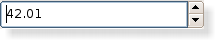
\includegraphics[scale=0.5]{graphics/spinbox}
			}
			\subfigure[A Combo Box]{
				\label{comboboxfig}
				
\includegraphics[scale=0.5]{graphics/combobox}
			}
			\subfigure[A Line Edit]{
				\label{lineeditfig}
				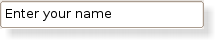
\includegraphics[scale=0.5]{graphics/lineedit}
			}
			\caption{Some of the various widgets used for editing data}
			\label{editingWidgets}
		\end{figure}

		\item QT was chosen as the GUI framework for several reasons:
			\begin{itemize}
				\item It is cross-platform.
				\item It is mature and has a well developed set of
				development tools.
				\item It has a rich feature-set.
				\item It has been used by Sandia in the past.
				\item The Optika developer was familiar with it.
			\end{itemize}
		\item Initially it was decided that the application developer would
		specify parameters via an XML file. A DTD would be created specifying
		the legal tags and name spaces.
		\item Dependencies would be handled through special tags in the DTD.
	\end{itemize}

\section{Early Development}
The first several months of development were spent on creating and implementing the XML
specification. The name of the XML specification went through several revisions but was
eventually called Dependent Parameter Markup Language (DPML).

After several months of development it was realized that creating an entirely new way of specifying 
parameters might hinder it's adoption. It pointed out that Trilinos actually had
a ParameterList~\cite{ParameterList} class in the Teuchos package. The ParameterList semmed to be better than DPML for
several reasons:
	\begin{itemize}
		\item It was already heavily adopted.
		\item It had the necessary hierarchical nature.
		\item It was serializable to and from XML.
	\end{itemize}

For these reasons, DPML was scrapted in favor of using Teucho's ParameterLists. Development moved
forward with the goal of creating a GUI framework that, in addiiton to meeting all the challenges 
outlined above, would also be compatiable with any existing program using Teuchos's ParameterLists.

\section{Heavy development}
Starting in May 2009 a more heavy focus was put on developement of the Trilinos GUI package.
With the backend data-structure of the Teuchos's ParameterList already in place, attention
was turned to the developing the actually GUI itself. A key technology provided by Qt was it's Model/View
framework~\cite{QtModelView}. Using the Model/View paradigm, a wrapper class named TreeModel
~\cite{TreeModel} was created around the ParameterList class by subclassing the 
QAbstractItemModel~\cite{QAbstractItemModel}.

However, in subclassing the QAbstractItemModel it was realized that the ParameterList class fell short in
certain areas. At this point the main issue was that a given ParameterEntry~\cite{ParameterEntry} located within
a ParameterList or a given sublist located within a ParameterList was not aware of it's parent.
This was an issue because Qt's Model/Veiw framework requires items within a model to be aware of
their parents. In order to circumvent this issue the TreeItem~\cite{TreeItem} class was created. Now 
instead of simply wrapping around a ParameterList class, the TreeModel created by giving it a ParameterList.
It would then read in the ParameterList and creat a structure of TreeItems.  Each TreeItem then contained a pointer 
to it's corresponding ParameterEntry.

Once the TreeModel and TreeItem class were complete an appropriate delegate to go between and View
and the TreeModel was needed. A new class called Delegate~\cite{Delegate} was created to fill this
role by subclassing QItemDelegate~\cite{QItemDelegate}. As specified above, the delegate would return
the apporiate editing widget based on it's datatype.

With the model and delegate classes inplace, an appropriate view could be applied. At first a simple
QTreeView~\cite{QTreeView} was applied to the model. The results was something like that in \ref{treeviewFig}.
	\begin{figure}[h]
		\centering
			\subfigure[A Tree View]{
				\label{treeviewFig}
				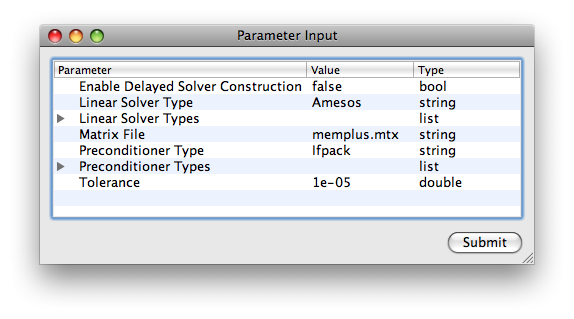
\includegraphics[scale=0.5]{graphics/treeview}
			}
	\end{figure}



\appendix
\section{Nomenclature}
    \begin{description}
	\item[Dependency]
	    A relationship between two or more parameters in which the state
		or value of one set of parameters depends on the state or value of
		another.
	\item[Dependee]
		The parameter upon which another parameter's state or value dependes.
	\item[Dependent]
		A parameter whose state or value is determined by another
		parameter.
	\item[Parameter]
	    An input needed for a program.
	\item[ParameterList]
	    A class containing a list of parameters and other parameter lists.
	\item[ParameterEntry]
		A class containing a parameter located in a ParameterList
	\item[RCP]
	    Refernce counted pointer. RCPs refered to in this document reference the
		RCP class located in the Teuchos~\cite{TeuchosPackage} package of Trilinos.
	\item[Sublist]
	    A parameter list contained within another parameter list.
	\item[Widget]
		A GUI element, usually used to obtain user input.
	\item[Validator]
		An object used to ensure a particular parameter's value is valid.
    \end{description}



\bibliographystyle{siam}
% Edit the line below to be your first and last names.
\bibliography{KurtisNusbaum,../OptikaSANDReport}
% Edit FirstnameLastname below to be your first and last names, but leave the line commented out.
% This line will help me merge bibliographies for the proceedings.
%\documentclass{csri10}

% PACKAGES ---------------------------------------------------------------
\usepackage{amsfonts,amsmath,graphicx,subfigure}
% ADD YOUR OWN PACKAGES HERE ---------------------------------------------
%\usepackage{someotherpackage}

% DEFINITIONS ------------------------------------------------------------
% ADD YOUR OWN DEFINITIONS HERE ------------------------------------------
% BE SURE TO PREFACE LABEL WITH YOUR OWN INITIALS (SSS in this example) --
\newcommand{\SSSnorm}[1]{\left\Vert#1\right\Vert}
\newcommand{\SSSabs}[1]{\left\vert#1\right\vert}

% This controls the table-of-contents entry in the proceedings. Edit it
% to include your article title followed by the authors' names, as shown.
\addcontentsline{toc}{chapter}{Optika: A GUI Framework for Parameterized Applications\\
{\em Kurtis Nusbaum Student and Dr.\ Mike Heroux Mentor}}

\pagestyle{myheadings}

\thispagestyle{plain}

% This gives the running head. Usually you list a shortened version of
% your article title (unless it's already very short) along with
% the author's names, as shown.
\markboth{Optika GUI Framework}{Kurtis Nusbaum Student and Dr.\ Mike Heroux Mentor}

% Put your article title in here
\title{Optika: A GUI Framework for Parameterized Applications}

% List each author, their affiliation, and their e-mail address, as shown.
\author{Kurtis L.\ Nusbaum\thanks{St. John's University, klnusbaum@csbsju.edu} \and Dr.\ Mike Heroux\thanks{Sandia National Laboratories,
maherou@sandia.gov}}

\begin{document}

\maketitle

% Include your abstract here.
\begin{abstract}
In the field of scientific computing there are many specialized programs designed for specific applications 
in areas like biology, chemistry, and physics. These applications are often very powerful and extraodinarily 
useful in their respective domains. However, many suffer from a common problem: a poor user interface. Many 
of these programs are homegrown, and the concern of the designer was not ease of use but rather 
functionality. The purpose of Optika is to address this problem and provide a simple, viable solution. Using
only a list of parameters passed to it, Optika can dynamically generate a GUI. This allows the user to specify 
parameters values in fashion that is much more intuitive than the traditional "input decks" used by many 
parameterized scientific applications. By leverageing the power of Optika, these scientific applications 
will become more accessible and thus allow their designers to reach a much wider audience while requiring 
minimal extra development effort.

\end{abstract}

\section{Introduction} \label{SSS:sec:intro}
I like chocolate pudding.  For that matter everyone else does too. This relationship is captured in \eqref{SSS:eq:one},
\begin{equation}\label{SSS:eq:one}
f(x) = x^{100-d},
\end{equation}
where $f$ is happiness in utils, $x$ is the quantity of chocolate pudding consumed in ounces and $d$ is the age of the
subject in years.

It has been argued that that chocolate pudding consumption by age is shown in Figure \ref{SSS:fig:Mentor05}.  However,
we propose an alternative pudding consumption model, shown in Figure \ref{SSS:fig:cos}.

\begin{figure}[hbh]
\begin{center}
\scalebox{0.5}{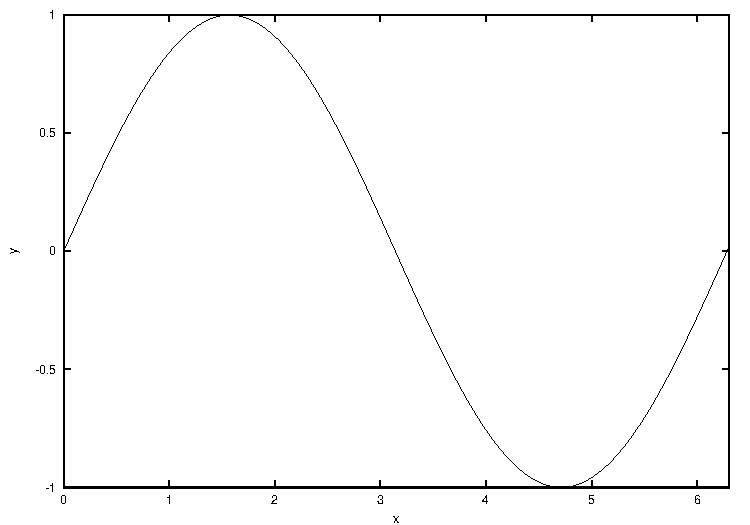
\includegraphics{plots/sinx}} \caption{Chocolate pudding consumption model of
\cite{SSS:Mentor05}}\label{SSS:fig:Mentor05}
\end{center}\end{figure}

\begin{figure}[htb]
\begin{center}
\scalebox{0.5}{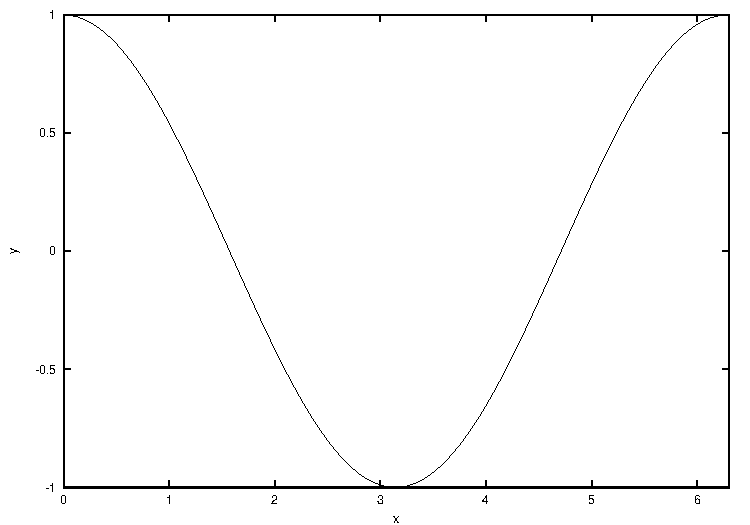
\includegraphics{plots/cosx}} \caption{Proposed chocolate pudding consumption model}\label{SSS:fig:cos}
\end{center}\end{figure}

We also want to show these figures side by side, to better illustrate our comparison.  We can see this in Figures
\ref{SSS:fig:comp1} and \ref{SSS:fig:comp2}.

\begin{figure}[htb]
\begin{center}
\subfigure[M. Mentor's Model]{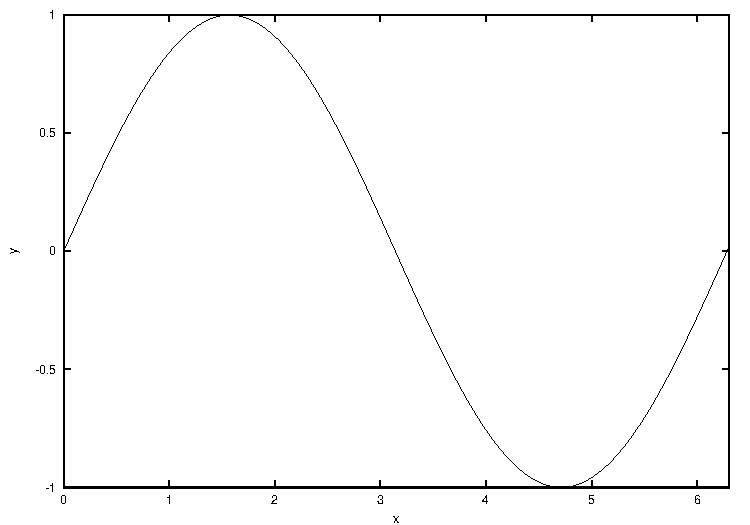
\includegraphics[scale=.5]{plots/sinx}\label{SSS:fig:comp1}} \subfigure[Proposed
Model]{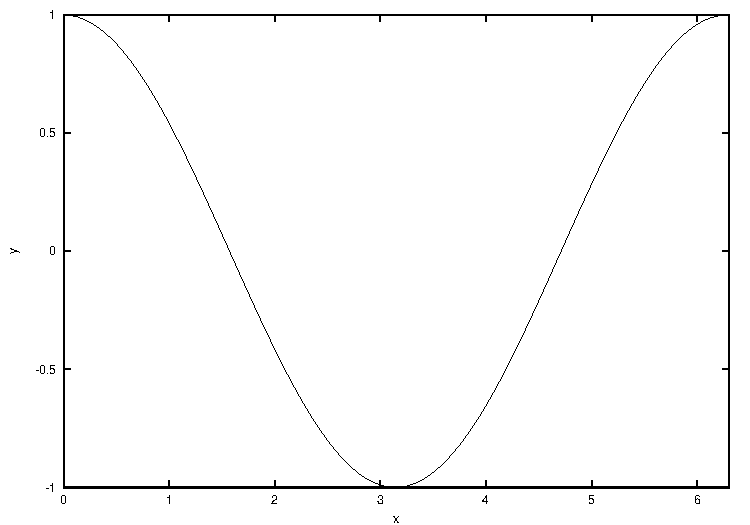
\includegraphics[scale=.5]{plots/cosx}\label{SSS:fig:comp2}} \caption{Comparative chocolate pudding consumption
models}
\end{center}\end{figure}

\section{Actual Content}

As we saw in Section \ref{SSS:sec:intro}, we all like chocolate pudding. This is where I wish
\textsf{$\setminus$jargonfill} worked. It would fill the page with meaningless technobabble so I could illustrate this
package. Instead, I'll talk about how to use quotations in latex. "Never use these quotations." ``Always use these,
instead.''

\section{Conclusions}
Herein, we repeat the abstract in past tense.

Unlike many other baked goods, chocolate pudding is subject to a myriad of interesting (and unique) effects on both the
meso and nano scales.  Understanding these phenomena is critical, not only to America's restaurant industry, but to
children everywhere.  We have examined these effects and have proposed new potential models which accurately capture
the material structure of chocolate pudding.

\bibliographystyle{siam}
% Edit the line below to be your first and last names.
\bibliography{FirstnameLastname}

% Edit FirstnameLastname below to be your first and last names, but leave the line commented out.
% This line will help me merge bibliographies for the proceedings.
%\input{FirstnameLastname/FirstnameLastname.bbl}

\end{document}


\end{document}
